\documentclass[a4paper, 10pt]{article}
\usepackage{../../CEDT-Homework-style}

\usepackage{amsmath}
\allowdisplaybreaks

\setlength{\headheight}{14.49998pt}

\begin{document}
\subject[2110203 - Computer Engineering Mathematics II]
\hwtitle{Stats 1}{}{Week 1}{6733172621 Patthadon Phengpinij}{ChatGPT (for\,\LaTeX\,styling and grammar checking)}


% ================================================================================ %
\section{Sampling}
% ================================================================================ %


Sampling is a process that is very important for writing simulations.
In this section, you will try to sample from some common distributions.
You may implement them yourself or use the provided distribution from \texttt{ scipy.stats }.

\begin{codingbox}
from scipy.stats import norm, bernoulli, binom, uniform, geom, expon

# Sample from Uniform(a, b)
def sample_uniform(sample_size, a, b):
  # [YOUR CODE HERE]
  dist = uniform(a, b)
  return dist.rvs(sample_size)

def sample_normal(sample_size, mu, sigma):
  # [YOUR CODE HERE]
  dist = norm(mu, sigma)
  return dist.rvs(sample_size)

def sample_bernoulli(sample_size, p):
  # [YOUR CODE HERE]
  dist = bernoulli(p)
  return dist.rvs(sample_size)

def sample_binomial(sample_size, n, p):
  # [YOUR CODE HERE]
  dist = binom(n, p)
  return dist.rvs(sample_size)

def sample_geometric(sample_size, p):
  # [YOUR CODE HERE]
  dist = geom(p)
  return dist.rvs(sample_size)

def sample_exponential(sample_size, l):
  # [YOUR CODE HERE]
  dist = expon(l)
  return dist.rvs(sample_size)
\end{codingbox}

\newpage

% ================================================================================ %
%                                  TO SUBMIT 01                                    %
% ================================================================================ %
\begin{tosubmit}
Hamtaro and his friends are collecting sunflower seeds. The bigger the sunflower, the more seeds they can find!
The probability of finding a sunflower of a certain height \( x \) (in cm, from 0 to 10) increases with its height, following the probability density function \( f(x)= \frac{x}{50} \).
Write a function \texttt{ sample\_increasing(sample\_size) } to simulate the heights of the sunflowers the Ham-Hams find.

\vspace{5mm}

\par\noindent\submitsolution
First, we need to find the cumulative distribution function (CDF) from the given probability density function (PDF) \( f(x) = \frac{x}{50} \).
To find the CDF, we integrate the PDF from 0 to \( x \):
\[
    F(x) = \int_0^x f(t) \, dt = \int_0^x \frac{t}{50} \, dt = \sqbracket{ \frac{t^2}{100} }_0^x = \frac{x^2}{100} \text{ for } 0 \leq x \leq 10.
\]
Next, we need to find the inverse of the CDF, \( F^{-1}(y) \), to use the inverse transform sampling method.
Setting \( y = F(x) \), we have:
\[
    y = \frac{x^2}{100} \implies x^2 = 100y \implies x = 10\sqrt{y}.
\]
Thus, the inverse CDF is \( F^{-1}(y) = 10\sqrt{y} \).

Now, we can implement the function \texttt{ sample\_increasing(sample\_size) } to generate random samples from the distribution.
\begin{codingbox}
import numpy as np

np.random.seed(1)  # For reproducibility

# sample from pdf f(x)=x/50, 0<=x<=10
def sample_increasing(sample_size):
  # [YOUR CODE HERE]
  u = np.random.rand(sample_size)
  dist = 10 * np.sqrt(u)
  return dist
\end{codingbox}

We can plot the histogram of our samples.
If the sample functions are implemented correctly, the histogram should looks like our distribution.
\begin{center}
    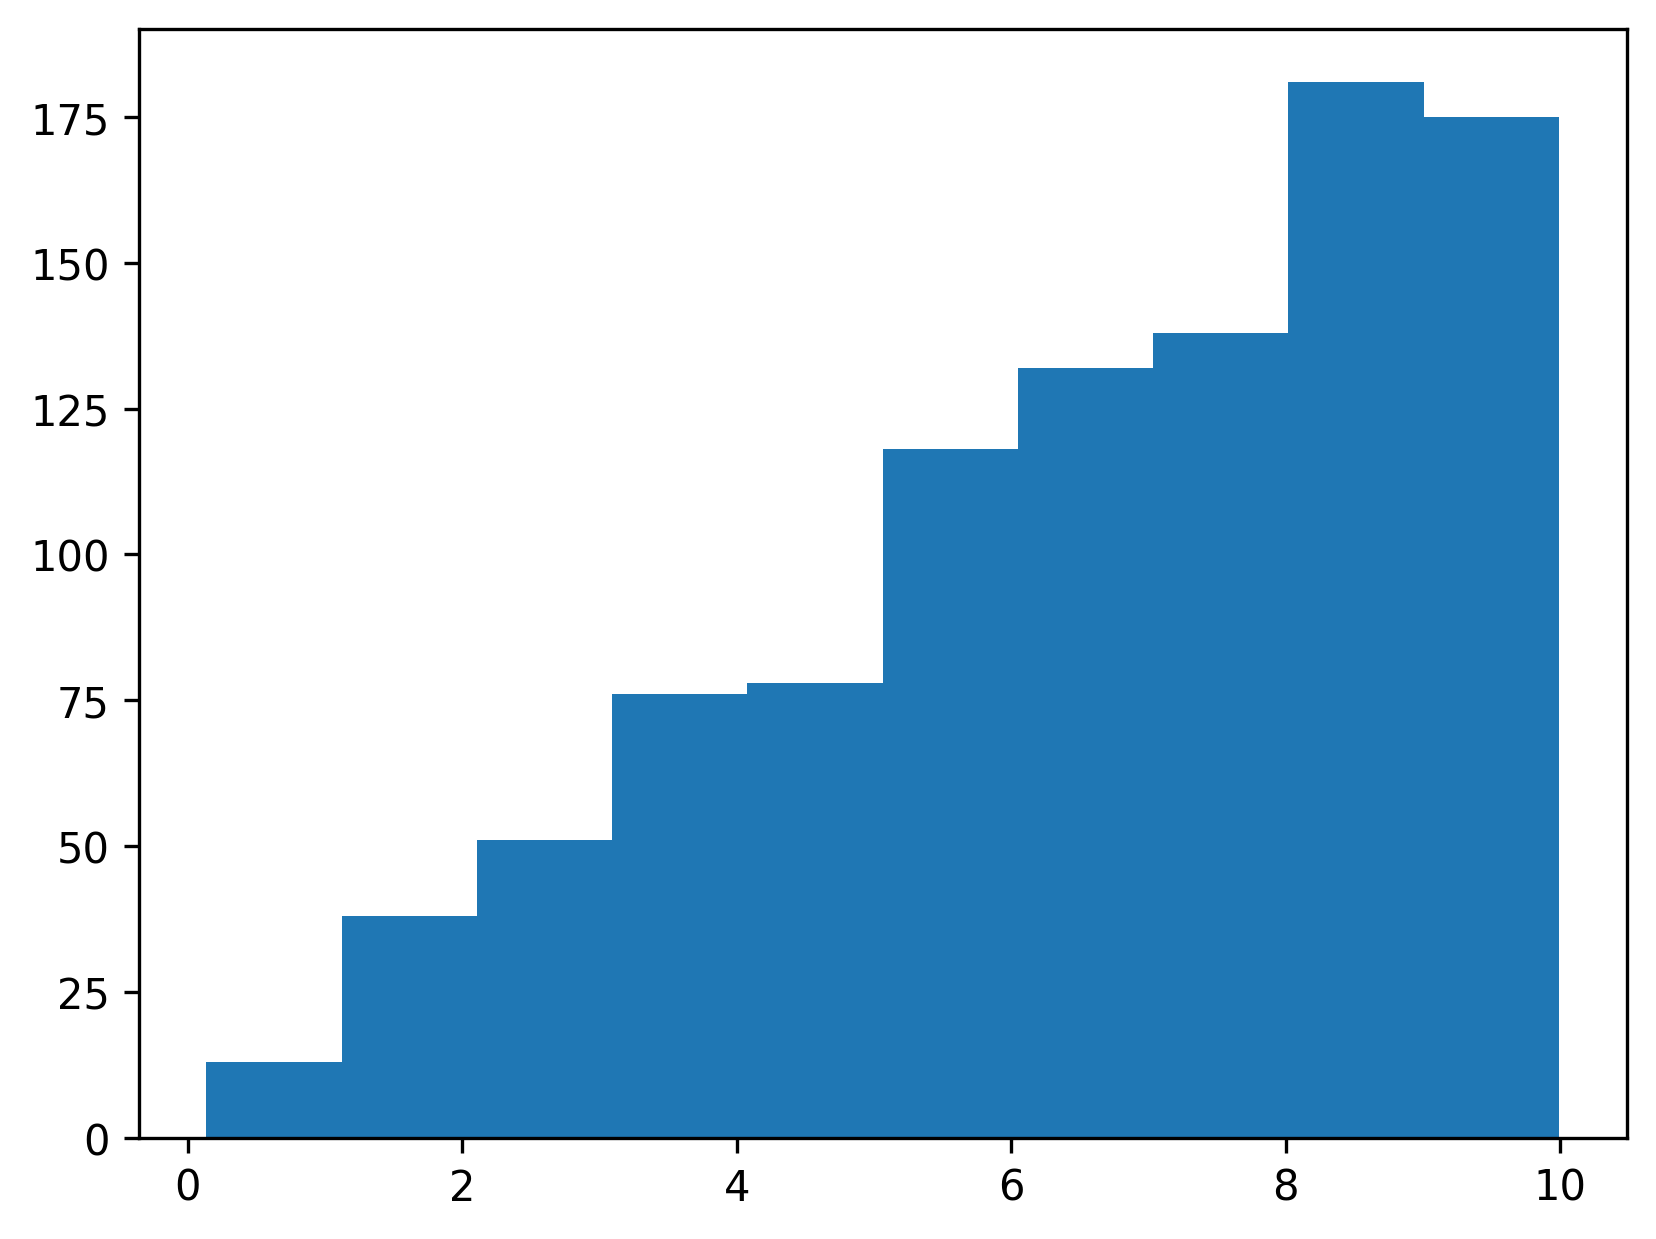
\includegraphics[width=0.6\textwidth]{images/sampling_increasing.png}
\end{center}
\end{tosubmit}
% ================================================================================ %

\newpage

% ================================================================================ %
%                                    Problem 00                                    %
% ================================================================================ %
\begin{problem}[0]
Try playing with the sample size and see how the histogram change with each run.
Check if the result match what you think. Explain in detail.
\end{problem}

\begin{solution}
When we increase the sample size, the histogram of the sampled data becomes smoother
and more closely resembles the theoretical probability density function (PDF) \( f(x) = \frac{x}{50} \).
This is due to the Law of Large Numbers, which states that as the number of trials increases,
the sample mean will converge to the expected value.

Using Python code, we can visualize this effect by plotting histograms for different sample sizes.
\begin{codingbox}
import matplotlib.pyplot as plt

np.random.seed(1)  # For reproducibility

Ns = [10, 100, 1000, 10000, 100000, 1000000]

# Create a 3x2 subplot grid
fig, axes = plt.subplots(3, 2, figsize=(12, 15))
axes = axes.flatten()  # Flatten to make indexing easier

for i, N in enumerate(Ns):
    data = sample_increasing(N)
    
    # Plot histogram on the corresponding subplot
    axes[i].hist(data, bins=30, density=True, alpha=0.6, color="g")

    # Plot the theoretical PDF
    x = np.linspace(0, 10, 100)
    pdf = x / 50
    axes[i].plot(x, pdf, "r-", lw=2, label="Theoretical PDF")

    axes[i].set_title(f"Histogram of Sample Size {N}")
    axes[i].set_xlabel("x")
    axes[i].set_ylabel("Density")
    axes[i].grid(True)
    axes[i].legend()

plt.tight_layout()
plt.show()
\end{codingbox}

\newpage

The following figure shows the histograms for different sample sizes.
\begin{center}
    \includegraphics[width=0.8\textwidth]{images/sampling_increasing_grid.png}
\end{center}

As we can see, with a small sample size (e.g., \( N = 10 \)), the histogram is quite irregular and does not closely follow the theoretical PDF.
However, as the sample size increases (e.g., \( N = 1000, 10000, 100000, 1000000 \)), the histogram becomes smoother and more closely matches the shape of the theoretical PDF.
\end{solution}
% ================================================================================ %

\newpage

% ================================================================================ %
\section{Maximum Likelihood Estimation}
% ================================================================================ %


% ================================================================================ %
%                                    Problem 01                                    %
% ================================================================================ %
\begin{problem}
Machines in Hamtaro's factory have their lifetime modelled by exponential distribution with an unknown parameter.
Hamtaro found out that his machines failed after \( x_1, x_2, ..., x_n \) years. Estimate the unknown parameter.
\end{problem}

\begin{solution}
The estimated parameter \( \lambda \) is calculated as the ratio of the number of observations \( n \) to the sum of the observed lifetimes \( \sum_{i=1}^{n} x_i \).
\[
    \hat{\lambda} = \frac{n}{\sum_{i=1}^{n} x_i}
\]

Using Python code, we can implement the MLE for the exponential distribution parameter \( \lambda \).
\begin{codingbox}
import numpy as np

machine_failed_time = [2, 3, 1, 3, 4]   # In class example
# machine_failed_time = sample_exponential(5, 0.3)  # Sampled from exponential distribution

def prob1_mle(X):
  return len(X)/np.sum(X)

print("The estimated parameter is: {}".format(prob1_mle(machine_failed_time)))
\end{codingbox}

For example, if the observed lifetimes of the machines are \( [2, 3, 1, 3, 4] \) years, the estimated parameter \( \lambda \) would be:
\[
    \hat{\lambda} = \frac{5}{2 + 3 + 1 + 3 + 4} = \frac{5}{13} \approx 0.3846
\]
\boxed{\text{The MLE } \hat{\lambda} \text{ is: } 0.3846}
\end{solution}
% ================================================================================ %

\newpage

% ================================================================================ %
%                                    Problem 02                                    %
% ================================================================================ %
\begin{problem}
Cappy is learning to perfectly replicate a new hat design.
The number of attempts he needs follows a Geometric distribution with unknown parameter.
For \( n \) different designs, he failed \( x_1, x_2, ..., x_n \) times before succeed.
Find the MLE of the parameter.
\end{problem}

\begin{solution}
The estimated parameter \( p \) is calculated as the ratio of the number of successes \( n \) to the total number of trials \( \sum_{i=1}^{n} x_i \).
\[
    \hat{p} = \frac{n}{\sum_{i=1}^{n} x_i}
\] 

Using Python code, we can implement the MLE for the geometric distribution parameter \( p \).
\begin{codingbox}
import numpy as np

X = [0, 0, 2] # In Class Example
# X = sample_geometric(10, 0.9)   # Sampled from actual geometric distribution

def prob2_mle(X):
  # [YOUR CODE HERE]
  return len(X)/np.sum(X)

print("The MLE is {}".format(prob2_mle(X)))
\end{codingbox}

For example, if the number of failures before success for different designs are \( [0, 0, 2] \), the estimated parameter \( p \) would be:
\[
    \hat{p} = \frac{3}{0 + 0 + 2} = \frac{3}{2} = 1.5
\]
\boxed{\text{The MLE } \hat{p} \text{ is: } 1.5}
\end{solution}
% ================================================================================ %

\newpage

% ================================================================================ %
%                                    Problem 03                                    %
% ================================================================================ %
\begin{problem}
Suppose our data \( x_1, x_2, ..., x_n \) is randomly drawn from uniform distribution \( U(a,b) \). Find MLE of \( a \) and \( b \).
\end{problem}

\begin{solution}
The estimated parameters \( \hat{a} \) and \( \hat{b} \) can be found using the following formulas:
\[
    \hat{a} = \min(x_1, x_2, ..., x_n)
\]
\[
    \hat{b} = \max(x_1, x_2, ..., x_n)
\]

Using Python code, we can implement the MLE for the uniform distribution parameters \( a \) and \( b \).
\begin{codingbox}
import numpy as np

X = sample_uniform(100, 60, 78)

def prob3_mle(X):
  # [YOUR CODE HERE]
  a = np.min(X)
  b = np.max(X) - a
  return a, b

a, b = prob3_mle(X)
print("The MLE is ({}, {})".format(a, b))
\end{codingbox}

By the code above, we can get the MLE of \( a \) and \( b \).
\[
    \hat{a} = \min(x_1, x_2, ..., x_n) = 61.2829
\]
\[
    \hat{b} = \max(x_1, x_2, ..., x_n) = 75.0727
\]
\boxed{\text{The MLE } (\hat{a}, \hat{b}) \text{ is: } (61.2829, 75.0727)}
\end{solution}
% ================================================================================ %


% ================================================================================ %
%                                    Problem 04                                    %
% ================================================================================ %
\begin{tosubmit}
\begin{problem}
Dexter tracks the growth of his prized sunflower over three days (day 0, 1, and 2).
He believes the sunflower's height at the end of each day \( y_{t+1} \) is its height from the previous day \( y_t \)
multiplied by a secret growth factor, \( \alpha \), plus some random daily noise.

\vspace{3mm}

For a two-day period, we can observe the following Markov process:
\[
    P(y_2, y_1, y_0 | \alpha) = P(y_2|y_1)P(y_1|y_0)P(y_0 |\alpha)
\]
\noindent where \( y_2 \sim \mathcal{N}(\alpha y_1, \sigma^2), y_1 \sim \mathcal{N}(\alpha y_0, \sigma^2), y_0 \sim \mathcal{N}(0,\lambda) \)

\vspace{3mm}

\noindent Find the Maximum Likelihood Estimate (MLE) for the secret growth factor, \( \alpha \), given the observed heights at the end of each day \( y_2,y_1,y_0 \).
In other words, compute for the value of \( \alpha \) that maximizes \( P(y_2,y_1,y_0|\alpha) \).
\end{problem}

\newpage

\par\noindent\submitsolution
The probability density functions for the normal distributions are given by:
\[
    P(y_2|y_1) = \frac{1}{\sqrt{2\pi\sigma^2}} e^{-\frac{(y_2 - \alpha y_1)^2}{2\sigma^2}}
\]
\[
    P(y_1|y_0) = \frac{1}{\sqrt{2\pi\sigma^2}} e^{-\frac{(y_1 - \alpha y_0)^2}{2\sigma^2}}
\]
\[
    P(y_0|\alpha) = \frac{1}{\sqrt{2\pi\lambda}} e^{-\frac{y_0^2}{2\lambda}}
\]

Thus, the joint probability is:
\begin{align*}
    P(y_2, y_1, y_0| \alpha) &= P(y_2|y_1)P(y_1|y_0)P(y_0| \alpha)\\
    &= \frac{1}{\sqrt{2\pi\sigma^2}} e^{-\frac{(y_2 - \alpha y_1)^2}{2\sigma^2}} \times \frac{1}{\sqrt{2\pi\sigma^2}} e^{-\frac{(y_1 - \alpha y_0)^2}{2\sigma^2}} \times \frac{1}{\sqrt{2\pi\lambda}} e^{-\frac{y_0^2}{2\lambda}}
\end{align*}

Using \textbf{log likelihood}, we have:
\[
    \ln(P(y_2|y_1)) = \ln(\frac{1}{\sqrt{2\pi\sigma^2}}) + \paren{ -\frac{(y_2-\alpha y_1)^2}{2\sigma^2} }
\]
\[
    \ln(P(y_1|y_0)) = \ln(\frac{1}{\sqrt{2\pi\sigma^2}}) + \paren{ -\frac{(y_1-\alpha y_0)^2}{2\sigma^2} }
\]
\[
    \ln(P(y_0|\alpha)) = \ln(\frac{1}{\sqrt{2\pi\lambda}}) + \paren{ -\frac{y_0^2}{2\lambda}}
\]

Therefore, the log-likelihood function is:
\[
    \ln(P(y_2, y_1, y_0| \alpha)) = \ln(P(y_2|y_1)) + \ln(P(y_1|y_0)) + \ln(P(y_0| \alpha))
\]
\[
    \implies \sqbracket{ \ln(\frac{1}{\sqrt{2\pi\sigma^2}}) + \ln(\frac{1}{\sqrt{2\pi\sigma^2}}) + \ln(\frac{1}{\sqrt{2\pi\lambda}}) } - \frac{(y_2-\alpha y_1)^2 + (y_1-\alpha y_0)^2}{2\sigma^2} - \frac{y_0^2}{2\lambda}
\]

To find the MLE of \( \alpha \), we take the derivative of the log-likelihood with respect to \( \alpha \) and set it to zero:
\begin{align*}
    \frac{\text{d}}{\text{d}\alpha}\ln(P(y_2, y_1, y_0| \alpha)) &= - \frac{-2y_1(y_2-\alpha y_1) -2y_0(y_1-\alpha y_0)}{2\sigma^2} \\
    &=  \frac{y_1(y_2-\alpha y_1) + y_0(y_1-\alpha y_0)}{\sigma^2} \\
    0 &= y_1(y_2-\alpha y_1) + y_0(y_1-\alpha y_0) \\
    \implies y_1(y_2-y_1\hat{\alpha}) &= -y_0(y_1-y_0\hat{\alpha}) \\
    y_1y_2 - y_1^2\hat{\alpha} &= -y_0y_1+y_0^2\hat{\alpha} \\
    \hat{\alpha}(y_1^2 + y_0^2) &= y_0y_1 + y_1y_2
\end{align*}

Therefore: \( \boxed{\implies \hat{\alpha} = \frac{y_0y_1 + y_1y_2}{y_1^2 + y_0^2}} \)
\end{tosubmit}
% ================================================================================ %

\newpage

% ================================================================================ %
\section{Maximum A Posteriori Estimation}
% ================================================================================ %


% ================================================================================ %
%                                    Problem 05                                    %
% ================================================================================ %
\begin{problem}
Hamtaro is trying to find acorns hidden by Boss. Boss has three favourite types of hiding sports:

\begin{itemize}
    \item Type A - P[Acorn] = \( c_a \)
    \item Type B - P[Acorn] = \( c_b \)
    \item Type C - P[Acorn] = \( c_c \)
\end{itemize}

\noindent Boss has a habit to use Type A \( p_a \) of the time, Type B \( p_b \) of the time, and Type C \( p_c \) of the time.
Find the MAP estimate for finding acorns at a new spot. Using the following data:
\begin{codingbox}
num_spot = 3
spot_acorn_prob = [0.8, 0.5, 0.4]   # From slide
spot_select_prob = [0.4, 0.4, 0.2]  # From slide
n = 5
h = 2
\end{codingbox}
\end{problem}

\begin{solution}
Firstly, implement the function to calculate the posterior probability of finding acorns at each type of hiding spot.
\begin{codingbox}
def spot_posterior(n, h, head_prob, select_prob):
  # [YOUR CODE HERE]
  return math.comb(n, h) * ((head_prob) ** h) * ((1 - head_prob) ** (n - h)) * select_prob
\end{codingbox}

Using the provided data, we can calculate the posterior probabilities for each type of hiding spot.
\begin{codingbox}
p_map = 0
p_map_val = 0
for i in range(num_spot):
  posterior = spot_posterior(n, h, spot_acorn_prob[i], spot_select_prob[i])
  print("Spot {} has posterior of {}".format(i, posterior))
  if posterior > p_map_val:
    p_map_val = posterior
    p_map = spot_acorn_prob[i]

print("The estimated parameter is {}".format(p_map))
\end{codingbox}

The result of this code will give us the posterior probabilities for each type of hiding spot and the MAP estimate for finding acorns at a new spot.
\begin{verbatim}
Spot 0 has posterior of 0.02047999999999999
Spot 1 has posterior of 0.125
Spot 2 has posterior of 0.06912
The estimated parameter is 0.5
\end{verbatim}

\boxed{\text{The MAP estimate for finding acorns at a new spot is: }0.5}
\end{solution}
% ================================================================================ %

\newpage

% ================================================================================ %
%                                    Problem 06                                    %
% ================================================================================ %
\begin{problem}
From \url{https://xkcd.com/1132/}.
Assume that chance of the sun actually explode is \( 10^{-6} \).
What are the chance that the machine said the sun exploded when it actually isn't?
\end{problem}

\begin{solution}
To solve this problem, we can simulate the scenario using Python code.

\begin{codingbox}
def calculate_posterior_prob_of_lie(sun_prior, lie_prob):
  """
  Calculates the posterior probability that the machine is lying (the event
  did not happen) given that the machine reported 'YES'.
  """
  truth_prob = 1 - lie_prob

  # P(A) - Prior probability of the event happening
  p_A = sun_prior
  # P(~A) - Prior probability of the event NOT happening
  p_not_A = 1 - p_A

  # P(B|A) - Likelihood of machine saying 'YES' if event happened (it tells the truth)
  p_B_given_A = 1 - lie_prob
  # P(B|~A) - Likelihood of machine saying 'YES' if event did not happen (it lies)
  p_B_given_not_A = lie_prob

  # P(B) - Total probability of the machine saying 'YES' (the evidence)
  # This is the sum of true positives and false positives.
  p_B = p_B_given_A * p_A + p_B_given_not_A * p_not_A

  # P(~A|B) - The posterior probability we want to find.
  # This is the probability of a false positive, given a positive result.
  p_not_A_given_B = p_B_given_not_A * p_not_A / p_B
  return p_not_A_given_B

  # Parameters from the problem
  sun_prior = 1e-6
  lie_prob = 1/36
  
  # Calculate and print the result
  chance_of_lie = calculate_posterior_prob_of_lie(sun_prior, lie_prob)
  print("Given the machine said 'YES'")
  print(f"The probability it's a false alarm is: {chance_of_lie:.8f}")
\end{codingbox}

The result of this code will give us the posterior probability that the machine is lying given that it reported 'YES'.
\begin{verbatim}
Given the machine said 'YES'.
The probability it's a false alarm is: 0.999965
\end{verbatim}
\end{solution}
% ================================================================================ %

\newpage

% ================================================================================ %
%                                    Problem 07                                    %
% ================================================================================ %
\begin{problem}
Go back to problem 1 - 2, and try to play with input size and parameter.
Observe the change in result.
Explain in detail.
\end{problem}

% === 7.1. === %
\begin{subproblems}
    \item \textbf{Problem 1: } Machines in Hamtaro's factory have their lifetime modelled by exponential distribution with an unknown parameter.
\end{subproblems}

\begin{solution}
This problem involves estimating the parameter \( \lambda \) of an exponential distribution for the different sample sizes.
\begin{codingbox}
import matplotlib.pyplot as plt
import numpy as np

sample_sizes = [10, 100, 1000, 10000, 100000]
true_param = 0.9

mles = np.ndarray(len(sample_sizes))

np.random.seed(1)

for i, sample_size in enumerate(sample_sizes):
    X = sample_geometric(sample_size, true_param)
    mle = prob2_mle(X)
    mles[i] = mle

plt.plot(sample_sizes, mles, marker="o", label="MLE Estimates")
plt.axhline(y=true_param, color="r", linestyle="--", label="True Parameter")
plt.xscale("log")
plt.xlabel("Sample Size (log scale)")
plt.ylabel("MLE Estimate of p")
plt.title("MLE Estimates vs Sample Size for Geometric Distribution")
plt.legend()
plt.grid(True)
plt.show()
\end{codingbox}

This experiment shows how the MLE estimate of the parameter \( p \) converges to the true parameter value as the sample size increases.

\vspace{3mm}

The following figure shows the MLE estimates for different sample sizes.
\begin{center}
    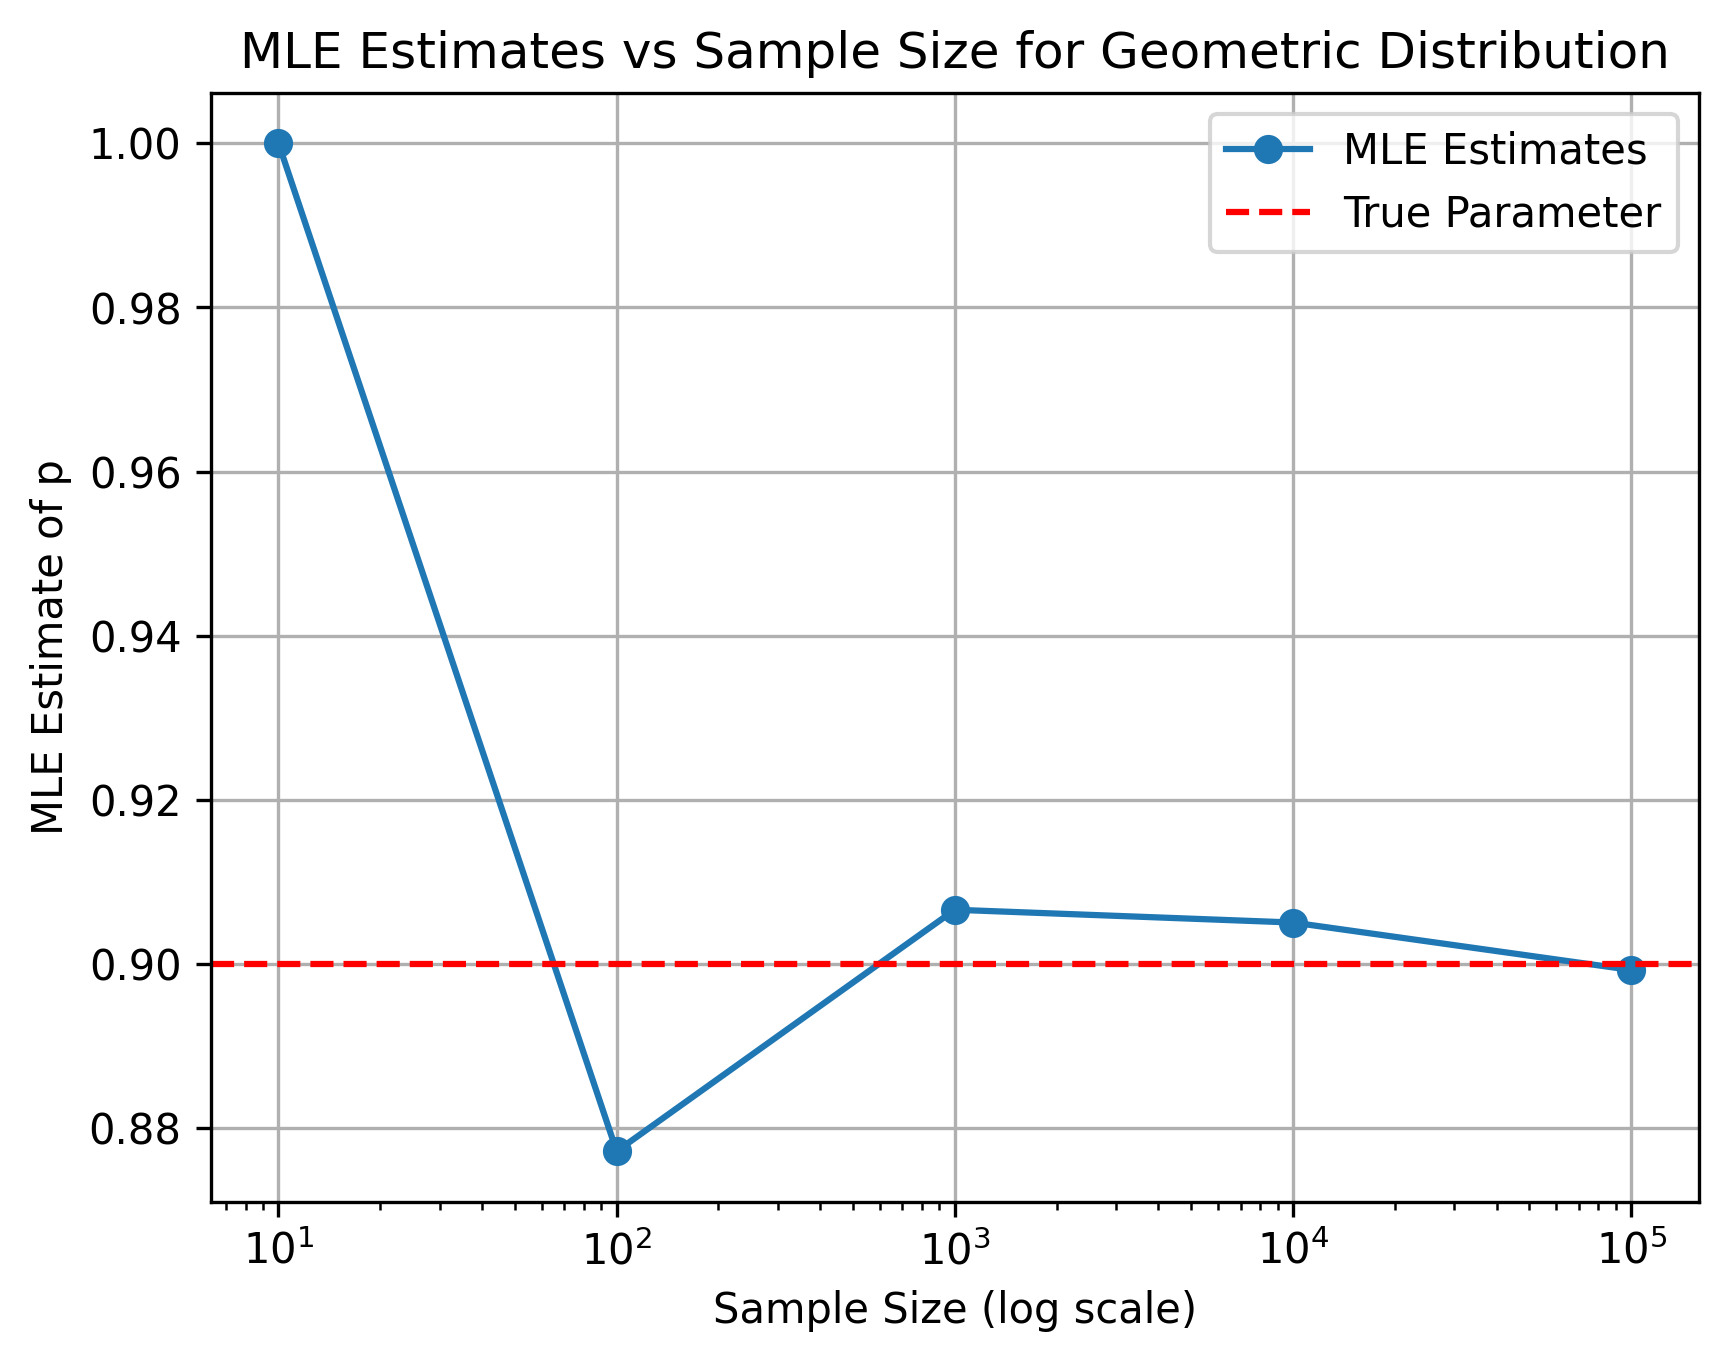
\includegraphics[width=0.5\textwidth]{images/problem_7_1.png}
\end{center}
\end{solution}
% ============ %

\newpage

% === 7.2. === %
\begin{subproblems}[start=2]
    \item \textbf{Problem 2: } Cappy is learning to perfectly replicate a new hat design.
\end{subproblems}

\begin{solution}
This problem involves estimating the parameter \( a, b \) of a uniform distribution for the different sample sizes.
\begin{codingbox}
import matplotlib.pyplot as plt
import numpy as np

sample_sizes = [10, 100, 1000, 10000, 100000]
true_param_a = 60
true_param_b = 78

mles = np.ndarray((len(sample_sizes), 2))

np.random.seed(1)

for i, sample_size in enumerate(sample_sizes):
    X = sample_uniform(sample_size, true_param_a, true_param_b)
    mle = prob3_mle(X)
    mles[i] = mle

fig, axes = plt.subplots(1, 2, figsize=(12, 5))
axes = axes.flatten()

for i, p in enumerate(["A", "B"]):
    axes[i].plot(sample_sizes, mles[:, i], marker="o", label=f"MLE Estimate of {p}")
    axes[i].axhline(y=[true_param_a, true_param_b][i], color="r", linestyle="--", label=f"True Parameter {p}")
    axes[i].set_xscale("log")
    axes[i].set_xlabel("Sample Size (log scale)")
    axes[i].set_ylabel(f"MLE Estimate of {p}")
    axes[i].set_title("MLE Estimates vs Sample Size for Uniform Distribution")
    axes[i].legend()
    axes[i].grid(True)

plt.show()
\end{codingbox}

Like the previous problem, this experiment shows how the MLE estimates of the parameters \( a \) and \( b \) converge to the true parameter values as the sample size increases.

\vspace{3mm}

The following figure shows the MLE estimates for different sample sizes.
\begin{center}
    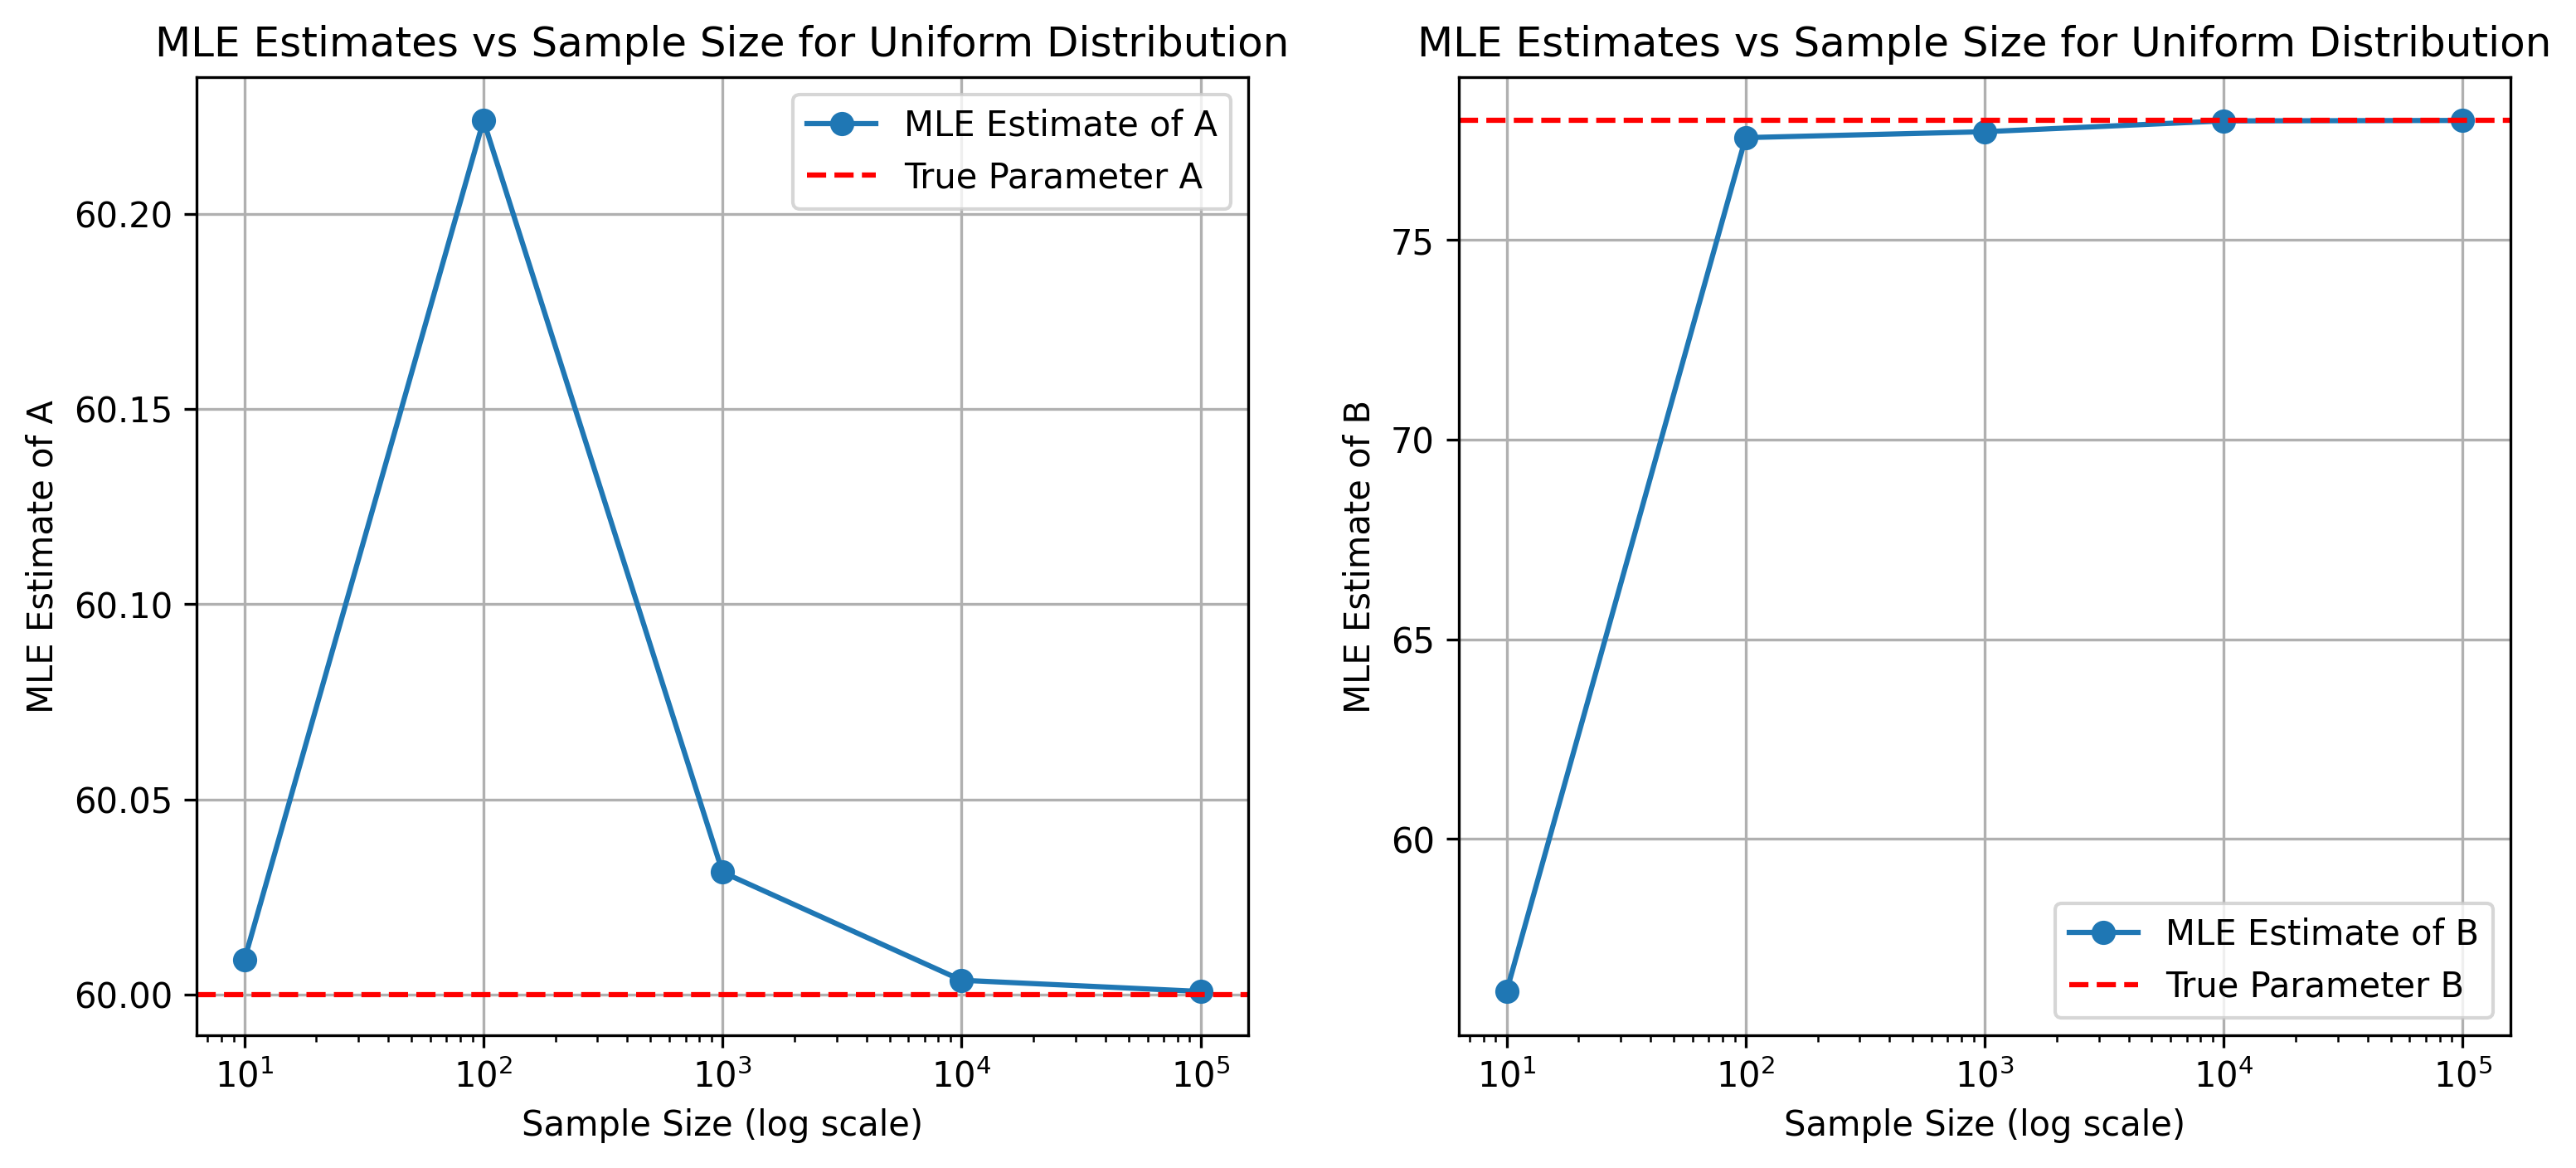
\includegraphics[width=0.7\textwidth]{images/problem_7_2.png}
\end{center}
\end{solution}
% ============ %
% ================================================================================ %

\end{document}